\section{Radiometría}
Radiometría es el campo dedicado al estudio y medición de la radiación electromagnética. Para el computo de la distribución de la luz es necesario entender algunas unidades importantes \cite{advanced_gi2006}.

\subsection{Unidades en Radiometría}

\subsubsection{Flujo Radiante}
La unidad fundamental en radiometría, usualmente denotada como $\Phi$ es expresada en watts o vatios. Esta cantidad expresa cuanta energía total fluye desde, hasta y a través de una superficie por unidad de tiempo.
\subsubsection{Irradiancia}
\label{subsubsec:irradiance}
La irradiancia $E$ es el flujo radiante entrante o incidente por unidad sobre el área de una superficie. Esta es expresada en $watts/m^2$:

\begin{equation}
    E = \frac{d\Phi}{dA}
	\label{eq:irradiance_eq}
\end{equation}

\subsubsection{Emitancia Radiante o Radiosidad}
La emitancia radiante $M$ es el flujo radiante saliente o emitido por unidad sobre el área de una superficie. También es expresada en $watts/m^2$:

\begin{equation}
    M = \frac{d\Phi}{dA}
	\label{eq:radiosity_eq}
\end{equation}

\subsubsection{Radiancia}
La radiancia $L$ es el flujo radiante emitido por unidad de ángulo sólido y por unidad de área proyectada, expresada en $watts/estereorradi\acute{a}n\cdot m^2$. De forma intuitiva la radiancia expresa cuanta potencia llega (o sale) de un punto $x$ por unidad de ángulo sólido y por unidad de área proyectada. La radiancia varia con la posición $x$ y el vector dirección $\Theta$, es expresada como $L(x,\Theta)$.

\begin{equation}
    L = \frac{d^2\Phi}{dwdA^\bot} = \frac{d^2\Phi}{dwA\cos\theta}
	\label{eq:radiance_eq}
\end{equation}

\begin{figure}[H]
	\centering
	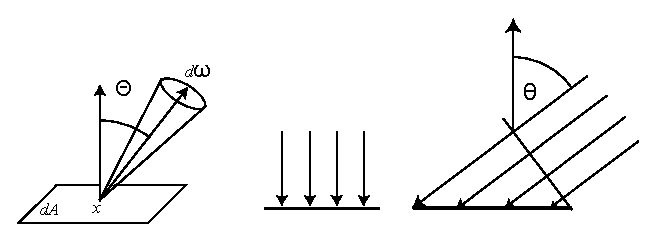
\includegraphics[width=0.85\linewidth]{media/radiance.eps}
	\caption{Definicion de radiancia $L(x,\Theta)$. Flujo radiante emitido por unidad de ángulo solido $dw$ y por unidad de área proyectada $A^\bot$.}
	\label{fig:radiance_fi}
\end{figure}

La radiancia es el término más importantes para los propósitos de este trabajo y probablemente lo es también para una cantidad importante de algoritmos y aproximaciones para el cálculo de iluminación global, es esta unidad la que captura la apariencia de los objetos en escena.
